%--------------------------------------------------------------
% - template for the main file of Informatica@Unifi Thesis 
% - based on Classic Thesis Style Copyright (C) 2008 
%   Andr\'e Miede http://www.miede.de   
%--------------------------------------------------------------
% Avoid warning
\RequirePackage{silence}
\WarningFilter{scrbook}{Usage of package `titlesec'}
\WarningFilter{scrbook}{Activating an ugly workaround}
\WarningFilter{scrbook}{\float@addtolist}
\WarningFilter{titlesec}{Non standard sectioning command detected}
%--------------------------------------------------------------
\documentclass[final,oneside,titlepage,fleqn,
	headinclude,12pt,a4paper,BCOR5mm,footinclude]{scrbook}
%--------------------------------------------------------------
\newcommand{\myItalianTitle}{MODELLI DI SISTEMI SEQUENZIALI E
CONCORRENTI\xspace} 
\newcommand{\myDegree}{Corso di Laurea Magistrale in Informatica\xspace}
\newcommand{\myName}{Marco Buracchi\xspace}
\newcommand{\myProf}{Prof. Rosario Pugliese\xspace}
\newcommand{\myFaculty}{
	Scuola di Scienze Matematiche, Fisiche e Naturali\xspace}
\newcommand{\myUni}{\protect{
	Universit\`a degli Studi di Firenze}\xspace}
\newcommand{\myLocation}{Firenze\xspace}
\newcommand{\myTime}{Anno Accademico 2015-2016\xspace} 
%--------------------------------------------------------------
\usepackage{dia-classicthesis-ldpkg}
%--------------------------------------------------------------
% Options for classicthesis.sty:
% tocaligned eulerchapternumbers drafting linedheaders 
% listsseparated subfig nochapters beramono eulermath parts 
% minionpro pdfspacing
\usepackage[eulerchapternumbers,linedheaders,subfig,beramono,eulermath,
parts]{classicthesis}
%--------------------------------------------------------------
\newcommand{\svar}{\textbf{S}}
\newcommand{\ssvar}{\textbf{SS}}
\newcommand{\sssvar}{\textbf{SSS}}
\newcommand{\ssssvar}{\textbf{SSSS}}
\newcommand{\sssssvar}{\textbf{SSSSS}}
\newcommand{\ssssssvar}{\textbf{SSSSSS}}
\newcommand{\sssssssvar}{\textbf{SSSSSSS}}
\newcommand{\kvar}{\textbf{K}}
\newcommand{\ivar}{\textbf{I}}
\newcommand{\aacc}{\`a\ }
\newcommand{\eacc}{\`e\ }
\newcommand{\iacc}{\`{\i}\ }
\newcommand{\oacc}{\`o\ }
\newcommand{\uacc}{\`u\ }
\renewcommand{\epsilon}{\varepsilon}
\renewcommand{\theta}{\vartheta}
\renewcommand{\rho}{\varrho}
\renewcommand{\phi}{\varphi}
%--------------------------------------------------------------
\usepackage[italian]{babel}
\usepackage[latin1]{inputenc} 
\usepackage[T1]{fontenc}
\usepackage[fleqn]{amsmath}
\usepackage{amssymb}
\usepackage{ellipsis}
\usepackage{subfig}
\usepackage{caption}
\usepackage{appendix}
\usepackage{siunitx}
\usepackage{stmaryrd}
\usepackage{tikz}
\usepackage[object=vectorian]{pgfornament}
\usepackage{listings}
\usepackage{mathpartir}
%--------------------------------------------------------------
\newlength{\abcd} % for ab..z string length calculation
% how all the floats will be aligned
\newcommand{\myfloatalign}{\centering} 
\setlength{\extrarowheight}{3pt} % increase table row height
\captionsetup{format=hang,font=small}
%--------------------------------------------------------------
% Layout setting
%--------------------------------------------------------------
\usepackage{geometry}
\geometry{
	a4paper,
	ignoremp,
	bindingoffset = 1cm, 
	textwidth     = 13.5cm,
	textheight    = 21.5cm,
	lmargin       = 3.5cm, % left margin
	tmargin       = 4cm    % top margin 
}

\lstset{
  	frame=tb,
	language=Matlab,
  	aboveskip=3mm,
  	belowskip=3mm,
  	showstringspaces=false,
  	columns=flexible,
  	basicstyle={\small\ttfamily},
  	numbers=none,
  	breaklines=true,
  	breakatwhitespace=true,
  	tabsize=3
}

\newcommand{\sectionline}{
	\begin{center}
		\resizebox{0.5\linewidth}{1ex}{
			\begin{tikzpicture}
				\node  (C) at (0,0) {};
				\node (D) at (9,0) {};
				\path (C) to [ornament=83] (D);
			\end{tikzpicture}
		}
	\end{center}
}
%--------------------------------------------------------------
\begin{document}
\frenchspacing
\raggedbottom
\pagenumbering{roman}
\pagestyle{plain}
%--------------------------------------------------------------
% Frontmatter
%--------------------------------------------------------------
%--------------------------------------------------------------
% titlepage.tex (use thesis.tex as main file)
%--------------------------------------------------------------
\begin{titlepage}
	\begin{center}
   	\large
      \hfill
      \vfill
      \begingroup
         
\includegraphics[scale=0.15]{logo/LOGO}\\
			\spacedallcaps{\myUni} \\ 
			\myFaculty \\
			\myDegree \\ 
			\vspace{0.5cm}
         \vspace{0.5cm}    
         Svolgimento esercizi assegnati    
      \endgroup 
      \vfill 
      \begingroup
      	\color{Maroon}\spacedallcaps{\myItalianTitle} \\ $\ $\\
      	\spacedallcaps{\myEnglishTitle}	
	\bigskip
      \endgroup
      \spacedlowsmallcaps{\myName}
      \vfill 
      \vfill
      \emph{\myProf}
      %Relatore: \emph{Andrea Bondavalli}\\
      %Correlatore: \emph{Andrea Ceccarelli}\\
      \vfill
      \vfill
      \myTime
      \vfill                      
	\end{center}        
\end{titlepage}   
%--------------------------------------------------------------
% back titlepage
%--------------------------------------------------------------
   \newpage
	\thispagestyle{empty}
	\hfill
	\vfill
	\noindent\myName: 
	\textit{\myItalianTitle,} 
	\myDegree, 
	%\textcopyright\ 
	\myTime
%--------------------------------------------------------------
% back titlepage end
%--------------------------------------------------------------
\tableofcontents
\pagenumbering{arabic}
\setcounter{secnumdepth}{0}
\chapter{Svolgimento esercizi assegnati}
	\section{Esercizio 2.13}
		\qquad Formalizzare e dimostrare la validit\`a dell'induzione strutturale
		\emph{mutua} che consente la dimostrazione simultanea di diverse propriet\`a
		per diverse categorie sintattiche.
		
		\sectionline
		
		\qquad A volte si ha la necessit\`a di dimostrare congiuntamente un gruppo di
		enunciati $S1(n),S2(n),\ldots,Sk(n)$ per induzione su n. Un gruppo di
		enunciati potrebbe essere dimostrato, dimostrando la congiunzione ($AND$
		logico) di tutti gli enunciati ($S1(n)\land S2(n)\land \ldots \land Sk(n)$).
		Tuttavia di solito conviene tenere separati gli enunciati e dimostrare per
		ciascuno la rispettiva base e il passo induttivo. Questo tipo di dimostrazione
		\`e detto \emph{induzione mutua}.
		
		Consideriamo ad esempio un interruttore on/off, rappresentato con il seguente
		automa:
		
		\begin{figure*}[h]
			\centering
			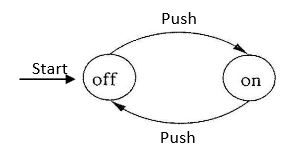
\includegraphics[scale=1]{img/Interruttore}
		\end{figure*}
		
		Ad ogni pressione del pulsante lo stato cambia tra ON e OFF. Proviamo a
		dimostrare i seguenti due enunciati:
		
		$S1(n):$ \emph{l'automa si trova nello stato OFF dopo n pressioni}
		$\Leftrightarrow$ \emph{n \`e pari.}
		
		$S2(n):$ \emph{l'automa si trova nello stato ON dopo n pressioni}
		$\Leftrightarrow$ \emph{n \`e dispari.}
		
		Sapendo che un numero $n$ non pu\`{o} essere allo stesso tempo pari e dispari, si
		potrebbe supporre che $S1 \Rightarrow S2$, e viceversa. Questo per\`{o} non \`{e}
		sempre vero in quanto, in generale, un automa potrebbe trovarsi
		contemporaneamente in pi\`{u} stati. Non \`{e} questo il caso dell'automa preso come
		esempio che si trova sempre esattamente in un solo stato, ma questo deve
		essere dimostrato come parte dell'induzione mutua.
		
		Proviamo a dimostrare le precedenti propriet\`a:
		
		\textbf{BASE:} Per il caso base scegliamo $n=0$. Dato che ci sono due
		enunciati, ognuno dei quali deve essere dimostrato in entrambe le
		direzioni ($S1$ e $S2$ sono enunciati `se e solo se`), in effetti ci sono
		quattro casi per la base e altrettanti per l'induzione:
		\begin{enumerate}
		  \item $[S1(0), \Rightarrow]$ Dato che $0$ \`e pari, dobbiamo dimostrare che dopo $0$
		  pressioni l'automa si trova nello stato OFF. Lo stato iniziale dell'automa \`e proprio
		  OFF e quindi l'automa si trova effettivamente nello stato OFF dopo $0$
		  pressioni.
		  \item $[S1(0), \Leftarrow]$ L'automa si trova nello stato OFF dopo $0$
		  pressioni, quindi dobbiamo dimostrare che $0$ \`e pari. $0$ \`e pari per
		  definizione quindi non resta altro da dimostrare.
		  \item $[S2(0), \Rightarrow]$ L'ipotesi afferma che $0$ \`e un numero dispari
		  $\Rightarrow$ l'implicazione \`e vera.
		  \item $[S2(0), \Leftarrow]$ L'ipotesi afferma che l'automa si trovi
		  nello stato ON dopo $0$ pressioni. Questo \`e impossibile in quanto all'automa
		  serve almeno una pressione del tasto per arrivare nello stato ON
		  $\Rightarrow$ l'implicazione \`e vera.
		\end{enumerate}
		
		\textbf{PASSO INDUTTIVO:} Supponiamo che $S1(n)$ e $S2(n)$ siano vere, e
		proviamo a dimostrare $S1(n+1)$ e $S2(n+1)$. Anche questa dimostrazione si divide in 4
		parti:
		
		\begin{enumerate}
		  \item $[S1(n+1), \Rightarrow]$ Per ipotesi, $n+1$ \`e pari. Di conseguenza $n$ \`e
		  dispari.
		  $S2(n)$ dice che dopo $n$ pressioni l'automa si trova nello stato ON. L'arco
		  da ON a OFF etichettato `Push` dice che la n+1-esima pressione far\`a
		  passare l'automa nello stato OFF.
		  \item $[S1(n+1), \Leftarrow]$ L'ipotesi \`e che l'automa si trovi nello
		  stato OFF dopo $n+1$ pressioni. Esaminando l'automa vediamo che l'unico modo
		  di pervenire allo stato OFF \`e di trovarsi nello stato ON e di ricevere in
		  input il comando `Push`. Perci\`{o}, se l'automa si trova nello stato OFF dopo
		  $n+1$ pressioni, deve essersi trovato nello stato ON dopo $n$ pressioni.
		  Quindi da $[S2(n), \Leftarrow]$ concludiamo che $n$ \`{e} dispari. Dunque
		  $n+1$ \`e pari.
		  \item $[S2(n+1), \Rightarrow]$ L'ipotesi afferma che $n+1$ \`e dispari. Di conseguenza
		  $n$ \`e pari. $[S1(n), \Rightarrow]$ dice che dopo $n$ pressioni l'automa si trova
		  nello stato OFF. L'arco da OFF a ON con etichetta `Push` dice che la
		  $n+1$-esima pressione far\`a passare l'automa nello stato ON.
		  \item $[S2(n+1), \Leftarrow]$ L'ipotesi \`e che l'automa si trovi nello
		  stato ON dopo $n+1$ pressioni. Esaminando l'automa vediamo che l'unico modo
		  di pervenire allo stato ON \`e di trovarsi nello stato OFF e di ricevere in
		  input il comando `Push`. Perci\`{o}, se l'automa si trova nello stato ON dopo
		  $n+1$ pressioni, deve essersi trovato nello stato OFF dopo $n$ pressioni.
		  Quindi da $[S1(n), \Leftarrow]$ concludiamo che $n$ \`{e} dispari. Dunque
		  $n+1$ \`{e} pari.
		\end{enumerate}
		
		Da questo esempio possiamo ricavare il modello di tutte le induzioni mutue:
		
		\begin{itemize}
		  \item Ogni enunciato deve essere dimostrato separatamente nella base e nel
		  passo induttivo.
		  \item Se si tratta di enunciati `se e solo se`, allora entrambe le direzioni
		  di ogni enunciato devono essere dimostrate, sia nella base che nel passo
		  induttivo.
		\end{itemize}
		
		\newpage
		
	\section{Esercizio 3.13}
		\qquad Fornire l'espressione, derivante dalla sintassi concreta
		dell'esercizio $11$, che ha il seguente albero di derivazione:
		
		\begin{figure*}[h]
			\centering
			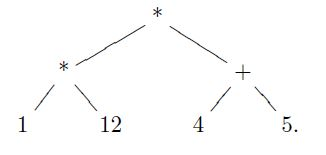
\includegraphics[scale=0.5]{img/3-13}
		\end{figure*}
		
		\sectionline
		
		\qquad L'espressione derivante \`e: $(1*12)*(4+5)$
		
		\newpage
	
	\newpage \section{Esercizio 4.6}
		\qquad Dimostrare che la semantica denotazionale delle espressioni regolari
		soddisfa le seguenti semplici propriet\`a:
		\subsection{punto (a)}
			$$E+(F+G) \simeq (E+F)+G$$
		\subsection{punto (e)}
			$$E(FG) \simeq (EF)G$$
		\subsection{punto (f)}
			$$E(F+G) \simeq EF+EG$$
		\subsection{punto (j)}
			$$E^* \simeq 1+E^*E$$
			
		\sectionline
		
		\qquad La semantica denotazionale delle espressioni regolari \`{e} cos\`{\i} definita:
		\begin{itemize}
		  \item $\mathcal{L} \llbracket 0 \rrbracket = \emptyset$
		  \item $\mathcal{L} \llbracket 1 \rrbracket = \{\epsilon\}$
		  \item $\mathcal{L} \llbracket a \rrbracket = \{a\}$ (per $a \in A$)
		  \item $\mathcal{L} \llbracket E + F \rrbracket = \mathcal{L} \llbracket E
		  	\rrbracket \cup \mathcal{L} \llbracket F
		  	\rrbracket$
		  \item $\mathcal{L} \llbracket E ; F \rrbracket = \mathcal{L} \llbracket E
		  	\rrbracket \cdot \mathcal{L} \llbracket F
		  	\rrbracket$ 
		  \item $\mathcal{L} \llbracket E^* \rrbracket = (\mathcal{L} \llbracket E
		  	\rrbracket)^*$ 
		\end{itemize}
		
		Da queste equivalenze possiamo ricavare:
		\begin{itemize}
		  \item punto (a):$$ E+(F+G) \simeq (E+F)+G $$  		  
		  	\begin{align*}
		  		\mathcal{L} \llbracket E+(F+G) \rrbracket &= \mathcal{L}
		  		\llbracket E \rrbracket \cup \mathcal{L}
		  		\llbracket F + G \rrbracket \\ &= \mathcal{L}
		  		\llbracket E \rrbracket \cup \mathcal{L}
		  		\llbracket F \rrbracket \cup \mathcal{L}
		  		\llbracket G \rrbracket \\ &= \mathcal{L}
		  		\llbracket E + F \rrbracket \cup \mathcal{L}
		  		\llbracket G \rrbracket \\ &= \mathcal{L} \llbracket (E + F) + G
		  		\rrbracket
		  	\end{align*}
		  \item punto (e): $$E(FG) \simeq (EF)G$$
		  	\begin{align*}
		  		\mathcal{L} \llbracket E(FG) \rrbracket &= \mathcal{L} \llbracket E
		  		\rrbracket \cdot \mathcal{L} \llbracket FG \rrbracket \\ &= \mathcal{L} \llbracket E \rrbracket \cdot
		  		\mathcal{L} \llbracket F \rrbracket \cdot \mathcal{L} \llbracket G
		  		\rrbracket \\ &= \mathcal{L} \llbracket EF \rrbracket \cdot \mathcal{L}
		  		\llbracket G \rrbracket \\ &= \mathcal{L} \llbracket (EF)G \rrbracket
		  	\end{align*}
		  \item punto (f): $$E(F+G) \simeq EF + EG$$
		  	\begin{align*}
		  		\mathcal{L} \llbracket E(F+G) \rrbracket &= \mathcal{L} \llbracket E
		  		\rrbracket \cdot \mathcal{L} \llbracket F+G \rrbracket \\ &= \mathcal{L} \llbracket E
		  		\rrbracket \cdot (\mathcal{L} \llbracket F \rrbracket \cup \mathcal{L}
		  		\llbracket G \rrbracket) \\ &= (\mathcal{L} \llbracket E \rrbracket \cdot
		  		\mathcal{L} \llbracket F \rrbracket) \cup (\mathcal{L} \llbracket E
		  		\rrbracket \cdot \mathcal{L} \llbracket G \rrbracket) \\ &= \mathcal{L}
		  		\llbracket EF + EG
		  		\rrbracket
		  	\end{align*}
		\end{itemize}
		
		\newpage
			
	\section{Esercizio 5.7}
	
		\qquad Siano:
		\begin{equation*}
			\svar = \lambda xyz.xz(yz)
		\end{equation*}
		\begin{equation*}
			\kvar = \lambda xy.x
		\end{equation*}
		\begin{equation*}
			\ivar = \lambda x.x
		\end{equation*}
		Trovare la forma normale dei due termini:
		\begin{equation*}
			(\lambda y.yyy)(\kvar\ivar)(\ssvar))\text{ e }\sssssssvar
		\end{equation*}
		
		\sectionline
		
		\begin{align*}
			(\lambda y.yyy)(\kvar\ivar(\ssvar)) & =
			\kvar\ivar(\ssvar)(\kvar\ivar(\ssvar))(\kvar\ivar(\ssvar))\\
			& = (\lambda y.\ivar)(\ssvar)((\lambda y.\ivar)(\ssvar))((\lambda
			y.\ivar)(\ssvar))\\
			& = \ivar\ivar\ivar\\
			& = \ivar\ivar\\
			& = \ivar\\
		\end{align*}
		
		\begin{align*}
			\sssssssvar & = (\lambda xyz.xz(yz))\ssssssvar\\
			& = (\lambda yz.\svar z(yz))\sssssvar\\
			& = (\lambda z.\svar z(\svar z))\ssssvar\\
			& = \ssvar(\ssvar)\sssvar\\
			& = (\lambda yz.\svar z(yz))(\ssvar)\sssvar\\
			& = (\lambda z.\svar z(\ssvar)z)\sssvar\\
			& = \ssvar(\sssvar)\ssvar\\
			& = (\lambda yz.\svar z(yz))(\sssvar)\ssvar\\
			& = (\lambda z.\svar z(\sssvar z))\ssvar\\
			& = \ssvar(\ssssvar)\svar\\
			& = (\lambda yz.\svar z(yz))(\ssssvar)\svar\\
			& \quad \vdots\\
			& = \lambda za.a a(a a(a a(\lambda b.b b(b b))))\\
		\end{align*}
		
		Lo svolgimento completo si trova in appendice A.
		
		\newpage
	
	\section{Esercizio 6.7}
		\qquad Risolvere le equazioni fra linguaggi:
		\begin{enumerate}
		  \item $X = \{a\} \cdot X$
		  \item $X = {a} \cup (\{b\} \cdot X)$
		\end{enumerate}
		dopo aver scelto gli opportuni domini e verificato che $\cdot$ e $\cup$ sono
		operazioni continue.
		
		\sectionline
		
		\begin{minipage}{0.2\linewidth}
			\begin{flushleft}
				$D:\{a,b\}$\\
				$\mathbb{D} = up(D)$\\
				$\mathbb{D}^*$
			\end{flushleft}
		\end{minipage}
		\hfill
		\begin{minipage}{0.7\linewidth}
			\begin{flushright}
				l'insieme composto dai caratteri 'a' e 'b'\\
				il dominio ottenuto tramite lifting da D\\
				il dominio sequenza di $\mathbb{D}$
			\end{flushright}
		\end{minipage}\\
		
		Dato che il membro sinistro \`e sempre composto da un solo carattere,
		possiamo definire la concatenazione $\cdot$ come il costruttore $\cdot ::
		\cdot$ e quindi affermarne la continuit\`a grazie al lemma $6.39$. L'unione
		$\cdot\cup\cdot$ pu\`{o} essere assimilata ad una somma disgiunta di domini
		considerando la somma disgiunta dei linguaggi.
		
		Le due equazioni generano i linguaggi $a^+$ e $b^*a$; sostituendo queste due
		espressioni nelle relative equazioni otteniamo infatti un'equivalenza. Le
		soluzioni delle equazioni sono dunque:
		
		\begin{enumerate}
		  \item $X = a^+$
		  \item $X = b^*a$
		\end{enumerate}
		
		\newpage
		
	\section{Esercizio 7.3}
		\qquad Introdurre in SLF un tipo di dato \emph{lista di naturali} e scrivere
		una funzione che, data una lista, ne calcola la lunghezza.
		
		\sectionline
		
		\subsection{Sintassi}
		
		\qquad Per introdurre il tipo di dati \emph{lista di naturali} abbiamo
		sicuramente bisogno di aggiungere i nuovi simboli $\{[,]\}$ e le nuove
		funzioni di base \textbf{hd}$(l)$, \textbf{tl}$(l)$, \textbf{null}$(l)$ e
		\textbf{remove}$(n,l)$ alla sintassi di SLF. Aggiungiamo ai valori di base il tipo di dato
		\emph{lista di naturali} $l := \{[n,l]\text{ }|\text{ }n \in
		\mathbb{NAT},l\text{ \`e una lista di naturali.}\}$
		
		Definiamo le funzioni di base che in generale si trovano associate alle
		liste:
		\begin{itemize}
		  \item $n\text{ }\textbf{::}\text{ }l$: questo \`e il costruttore che aggiunge
		  $n$ in testa alla lista $l$.
		  \item \textbf{hd}$(l)$: questa funzione restituisce il primo elemento della
		  lista (senza rimuoverlo).
		  \item \textbf{tl}$(l)$: questa funzione restituisce l'ultimo elemento della
		  lista (senza rimuoverlo).
		  \item \textbf{null}$(l)$: questa funzione restituisce $0$ (\emph{true})
		  se la lista \`e vuota o un numero $n+1$ (\emph{false}) altrimenti.
		  \item \textbf{remove}$(n,l)$: questa funzione rimuove la prima occorrenza dell'elemento $n$ dalla lista $l$ e restituisce la lista risultante
		\end{itemize}

		Con queste aggiunte, la nuova sintassi di SLF diventa la seguente:
		
		\begin{align*}
			P & ::= \textbf{letrec} \, D \, \textbf{in} \, T\\
			B & ::= n \, | \, l\\
			T & ::= x_i \, | \, B \, | \, \text{b}_j(T_1,\dots,T_m) \, | \, \text{f}_r(T_1,\dots,T_{\rho(r)}) \, | \, \textbf{if} \, T \, \textbf{then} \, T1 \, \textbf{else} \, T_2\\
			D & ::= \text{f}_1(x_1,\dots,x_{\rho(1)})\Leftarrow T_1,\dots,\text{f}_n(x_1,\dots,x_{\rho(n)}) \Leftarrow T_n\\ 
		\end{align*}
		\vspace{-16 mm}
		\begin{flushright}
			$\rho(j)$ \`{e} l'ariet\`{a} di $f_j$, $1\leq j\leq n$
		\end{flushright}
		
		\subsection{Semantica operazionale}
		
		\qquad Avendo aggiunto un tipo di dato di base, la semantica operazionale deve prevedere che si possano valutare funzioni che abbiano, come argomenti, anche le liste oltre ai naturali. Per questo motivo la regola di inferenza $(Bas_1)$ diventa:\\
		\begin{minipage}{0.7\linewidth}
			\vspace{5 mm}
			$\inferrule
				{ }
				{\text{b}_j(B_1,\dots,B_m) \rightarrow_D \, B}
				\quad b_j(B_1,\dots,B_m) = B$
		\end{minipage}
		\hfill
		\begin{minipage}{0.2\linewidth}
			\vspace{5 mm}
			\begin{flushright}
				$(Bas_1)$\\
			\end{flushright}
		\end{minipage}
		
		\subsection{Semantica denotazionale}
		
		\qquad Sicuramente la semantica denotazionale ha bisogno di qualche modifica in pi\`{u}, a partire dai tipi delle funzioni semantiche. Dobbiamo considerare che adesso i programmi (risp. i termini) possono restituire liste (possono essere composti da liste) e il dominio $(\mathbb{FUN}_m)^n$ rappresenter\`{a} il dominio delle funzioni continue con $m$ argomenti che potranno essere naturali o liste. Per questi motivi i nuovi tipi saranno i seguenti:
		
		\begin{align*}
		\mathcal{P} & : \, \emph{Prog}\rightarrow (\mathbb{NAT}+\mathbb{LIST})\\
		\mathcal{D} & : \, \emph{Decl}\rightarrow (\mathbb{FUN}_m)^n\\
		\mathcal{T} & : \, \emph{Term}\rightarrow (\mathbb{FUN}_m)^n \rightarrow (\mathbb{NAT} + \mathbb{LIST})^m\rightarrow (\mathbb{NAT}+\mathbb{LIST})\\
		\mathcal{B} & : \, \emph{Base} \rightarrow (\mathbb{NAT}+\mathbb{LIST})\\
		\end{align*}
		
		La semantica denotazionale, a questo punto, ha bisogno dell'aggiunta delle funzioni di interpretazione per la nuova classe sintattica $B$:
		
		\begin{align*}
		\mathcal{B} \llbracket n \rrbracket & = n\\
		\mathcal{B} \llbracket l \rrbracket & = l\\
		\mathcal{T} \llbracket B \rrbracket & = \lambda \overrightarrow{F}.\lambda \overrightarrow{X}.\mathcal{B} \llbracket B \rrbracket\\		
		\end{align*}
		
		\subsection{Funzione}
		\qquad La funzione richiesta pu\`o essere implementata come segue:
		
		$$\textbf{f}(l) \Leftarrow \textbf{if}\text{ }\textbf{null}(l)\text{
		}\textbf{then}\text{ }0\text{ }\textbf{else}\text{ }1 +
		\textbf{f}(\textbf{remove}(\textbf{hd}(l),l))$$
		
		\newpage
		
	\section{Esercizio 10.2}
		\qquad Si scriva un termine che descriva un distributore automatico in grado
		di offrire acqua o cioccolato un numero illimitato di volte, senza accettare
		monete fino a che non \`e stato servito l'utente precedente. Si risolva
		l'esercizio in tre modi: con l'operatore di ricorsione, con la definizione di
		costanti di processo e con l'operatore di replicazione.
		
		\sectionline
		
		\subsection{Operatore di ricorsione}
		
		\qquad Utilizzando l'operatore di ricorsione il termine richiesto pu\`{o} essere cos\`{\i} definito:
		
		$$D \triangleq rec.X.coin.(\overline{choc}.X\ \square \ \overline{water}.X)$$
		
		Si pu\oacc verificare che le possibili computazioni non accettano monete prima che il prodotto venga effettivamente ritirato. Una delle computazioni possibili, infatti, \eacc la seguente:
		
		\begin{minipage}{0.5\linewidth}
			\vspace{5mm}
			\begin{flushleft}
				$rec.X.coin.(\overline{choc}.X\ \square \ \overline{water}.X)$\\
				\vspace{10 mm}
				$\overline{choc}.rec.X.coin.(\overline{choc}.X\ \square \ \overline{water}.X)$\\
				$\qquad\square$\\
				$\overline{water}.rec.X.coin.(\overline{choc}.X\ \square \ \overline{water}.X)$\\
			\end{flushleft}
		\end{minipage}
		\hfill
		\begin{minipage}{0.4\linewidth}
			\begin{flushright}
				\vspace{5mm}
				$\xrightarrow{coin}$\\
				\vspace{9 mm}
				$\begin{cases}
					\text{in questo momento non accetta}\\
					\text{una nuova moneta finch\eacc non viene}\\
					\text{richiesta l'acqua o il cioccolato}\\
				\end{cases}$
			\end{flushright}
		\end{minipage}
		
		\subsection{Costanti di processo}
		
		\qquad Se vogliamo risolvere il problema utilizzando costanti di processo, la logica resta la stessa. Definendo la costante $D$ come
		$$D \triangleq coin.(\overline{choc}.D\ \square \ \overline{water}.D)$$ il risultato ottenuto \eacc identico. La computazione risultante infatti \eacc:
		
		\begin{minipage}{0.5\linewidth}
			\begin{flushleft}
				$coin.(\overline{choc}.D\ \square \ \overline{water}.D)$\\
				\vspace{18mm}
				$(\overline{choc}.D\ \square \ \overline{water}.D)$\\
			\end{flushleft}
		\end{minipage}
		\hfill
		\begin{minipage}{0.4\linewidth}
			\begin{flushright}
				\vspace{10mm}
				$\xrightarrow{coin}$\\
				\vspace{10mm}
				$\begin{cases}
				\text{come sopra, non accetta}\\
				\text{una nuova moneta finch\eacc non viene}\\
				\text{richiesta l'acqua o il cioccolato}\\
				\end{cases}$
			\end{flushright}
		\end{minipage}
		
		\subsection{Operatore di replicazione}
		
		\qquad Similare \eacc anche la soluzione che prevede l'utilizzo dell'operatore di replicazione. Definiamo $D$ come
		$$D \triangleq (\overline{a}\ |\ !a.coin.(\overline{choc}.\overline{a}\ \square\ \overline{water}.\overline{a}))\backslash a$$ e vediamo ad esempio una possibile computazione:
		
		\begin{minipage}{0.5\linewidth}
			\begin{flushleft}
				\vspace{5mm}
				$(\overline{a}\ |\ !a.coin.(\overline{choc}.\overline{a}\ \square\ \overline{water}.\overline{a}))\backslash a$\\
				\vspace{5mm}
				$coin.(\overline{choc}.\overline{a}\ \square\ \overline{water}.\overline{a}))\ |\ !a.coin.(\overline{choc}.\overline{a}\ \square\ \overline{water}.\overline{a}))\backslash a$\\
				\vspace{5mm}
				$((\overline{choc}.\overline{a}\ \square\ \overline{water}.\overline{a})\ |\ !a.coin.(\overline{choc}.\overline{a}\ \square\ \overline{water}.\overline{a}))\backslash a$
			\end{flushleft}
		\end{minipage}
		\hfill
		\begin{minipage}{0.4\linewidth}
			\begin{flushright}
				\vspace{5mm}
				$\xrightarrow{\tau}$\\
				\vspace{5mm}
				$\xrightarrow{coin}$\\
				\vspace{5mm}
				(come sopra)
			\end{flushright}
		\end{minipage}
		
		\newpage
		
	\section{Esercizio 11.3}
		\qquad Utilizzando la caratterizzazione delle simulazioni forti vista
		nell'Esercizio $11.1$, si provi che \emph{Id} \`e una simulazione e che se
		\emph{R} ed \emph{S} sono simulazioni allora $\emph{R} \cup \emph{S}$ ed
		\emph{RS} sono simulazioni.
		
		\sectionline
		
		\qquad Svolgimento\ldots\ldots\ldots
		
		\newpage
		
	\section{Esercizio 11.8}
		\qquad Dimostrare che l'unione di tutte le bisimulazioni di branching \`e una
		bisimulazione di branching e che essa \`e un'equivalenza.
		
		\sectionline
		
		\qquad Svolgimento\ldots\ldots\ldots
		
		\newpage
		
	\section{Esercizio 12.3}
		\qquad Relativamente alla definizione di insieme saturato (Definizione
		$12.57$), si dimostri che se $\mathcal{L}$ \`e saturato,allora valgono le
		seguenti propriet\`a:
		\begin{enumerate}
		  \item se $L_1,L_2 \in \mathcal{L}$ allora:
		  \begin{itemize}
		    \item $L_1 \cup L_2 \in \mathcal{L}$
		    \item se $L_1 \subseteq K \subseteq L_2$ allora $K \in \mathcal{L}$
		  \end{itemize}
		  \item \emph{Act}($\mathcal{L}$) $\in \mathcal{L}$
		\end{enumerate}
		
		\sectionline
		
		\qquad Svolgimento\ldots\ldots\ldots
\begin{appendices}
	\chapter{Svolgimento completo esercizio 5.7}

	\begin{align*}
		\sssssssvar & = (\lambda xyz.xz(yz))\ssssssvar\\
		& = (\lambda yz.\svar z(yz))\sssssvar\\
		& = (\lambda z.\svar z(\svar z))\ssssvar\\
		& = \ssvar(\ssvar)\sssvar\\
		& = (\lambda yz.\svar z(yz))(\ssvar)\sssvar\\
		& = (\lambda z.\svar z(\ssvar)z)\sssvar\\
		& = \ssvar(\sssvar)\ssvar\\
		& = (\lambda yz.\svar z(yz))(\sssvar)\ssvar\\
		& = (\lambda z.\svar z(\sssvar z))\ssvar\\
		& = \ssvar(\ssssvar)\svar\\
		& = (\lambda yz.\svar z(yz))(\ssssvar)\svar\\
		& = (\lambda z.\svar z(\ssssvar z))\svar\\
		& = \ssvar(\sssssvar)\\
		& = (\lambda yz.\svar z(yz))(\sssssvar)\\
		& = \lambda z.\svar z(\sssssvar z)\\
		& = \lambda z.(\lambda ya.a a(y a))(\sssssvar z)\\
		& = \lambda za.a a(\sssssvar a a)\\
		& = \lambda za.a a((\lambda yb.\svar b(y b))\sssvar z z)\\
		& = \lambda za.a a ((\lambda b.\svar b (\svar b)) \ssvar z z)\\
		& = \lambda za.a a (\ssvar (\ssvar) \svar a a)\\
		& = \lambda za.a a ((\lambda yb.\svar b (y b)) (\ssvar) \svar z z)\\
		& = \lambda za.a a ((\lambda b.\svar b (\ssvar b)) \svar z z)\\
		& = \lambda za.a a (\ssvar (\sssvar) a a)\\
		& = \lambda za.a a ((\lambda yb.\svar b (y b)) (\sssvar) z z)\\
		& = \lambda za.a a ((\lambda b.\svar b (\sssvar b)) z z)\\
		& = \lambda za.a a (\svar a (\sssvar a) a)\\
		& = \lambda za.a a ((\lambda yb.b b (y b)) (\sssvar z) z)\\
		& = \lambda za.a a ((\lambda b.b b (\sssvar b b)) z)\\
	\end{align*}
	\begin{align*}
		& = \lambda za.a a (a a (\sssvar a a))\\
		& = \lambda za.a a (a a ((\lambda yb.\svar b (y b)) \svar z z))\\
		& = \lambda za.a a (a a ((\lambda b.\svar b (\svar b)) z z))\\
		& = \lambda za.a a (a a (\svar a [\svar a] a))\\
		& = \lambda za.a a (a a ((\lambda yb.b b (y b)) (\svar z) z))\\
		& = \lambda za.a a (a a ((\lambda b.b b (\svar b b)) z))\\
		& = \lambda za.a a (a a (a a (\svar a a)))\\
		& = \lambda za.a a (a a (a a ((\lambda yb.b b (y b)) z)))\\
		& = \lambda za.a a (a a (a a (\lambda b.b b (b b))))\\
	\end{align*}
	
\end{appendices}
\pagestyle{scrheadings}
%--------------------------------------------------------------
% Mainmatter
%--------------------------------------------------------------

		
%--------------------------------------------------------------
\end{document}
%--------------------------------------------------------------
